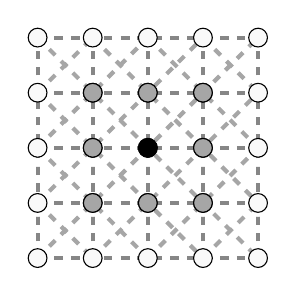
\begin{tikzpicture}[scale=0.7]
\foreach \x in {0,...,4}{
  \draw[dashed, line width=1.5pt, gray!95] (\x,0) to[out=90,in=-90] (\x,4);
  \draw[dashed, line width=1.5pt, gray!95] (0,\x) to[out=0,in=180] (4,\x);
}

\foreach \x in {1,...,3}{
  \draw[dashed, line width=1.5pt, gray!70] (0,\x) to[out=-45,in=135] (\x,0);
  \draw[dashed, line width=1.5pt, gray!70] (\x,4) to[out=-45,in=135] (4,\x);
  \draw[dashed, line width=1.5pt, gray!70] (\x,0) to[out=45,in=225] (4,4-\x);
  \draw[dashed, line width=1.5pt, gray!70] (0,\x) to[out=45,in=225] (4-\x,4);
}

\draw[dashed, line width=1.5pt, gray!70] (0,0) to[out=45,in=225] (4,4);
\draw[dashed, line width=1.5pt, gray!70] (0,4) to[out=-45,in=135] (4,0);

\foreach \x in {0,...,4} 
	\foreach \y in {0,...,4}
   		\draw[fill = gray!5] (\x,\y) circle (1.7mm); 

\draw[fill = black] (2,2) circle (1.7mm); 
\draw[fill = gray!70] (2,3) circle (1.7mm); 
\draw[fill = gray!70] (1,2) circle (1.7mm); 
\draw[fill = gray!70] (3,2) circle (1.7mm); 
\draw[fill = gray!70] (2,1) circle (1.7mm); 
\draw[fill = gray!70] (1,3) circle (1.7mm); 
\draw[fill = gray!70] (3,3) circle (1.7mm); 
\draw[fill = gray!70] (1,1) circle (1.7mm); 
\draw[fill = gray!70] (3,1) circle (1.7mm); 

\end{tikzpicture}